%%!TEX encoding = UTF-8 Unicode

\documentclass[a4paper,12pt]{article}
\usepackage{geometry}
\usepackage{graphicx}
\usepackage{amsmath}
\usepackage{amssymb}
\usepackage{xspace}
\usepackage{tikz,ifthen,fullpage}
\usepackage{xcolor}
\usepackage{sistyle}
\usepackage{epstopdf}
\usepackage[frenchb]{babel}
\usepackage[utf8]{inputenc}
\usepackage[T1]{fontenc}
\usepackage{listings}
\geometry{dvips,a4paper,margin=1.5in}
\DeclareGraphicsRule{.tif}{png}{.png}{`convert #1 `dirname #1`/`basename #1 .tif`.png}

\title{Etude des trajectoires électroniques dans un guide par la méthode des éléments finis}
\author{Elie Génard, Félix Tora}
\date{Mai 2013}


\begin{document}
\maketitle

Un électron soumis à un champ électromagnétique est soumis à la force de Lorentz qui contient une composante due au champ électrique et une autre due au champ magnétique. Seule la partie électrique est capable de fournir du travail à l'électron et donc de l'accélérer. Un électron dans un champ électrique a donc une trajectoire qui dépend à la fois des conditions initiales (position et vitesse) et du champ électrique appliqué.

\section{Position du probléme}

Le systéme étudié est un guide d'électrons. Des électrons sont émis depuis une source et sont "guidés" jusqu'à un détecteur dans un systéme coaxial. Le guide est constitué d'un fil porté au potentiel $V_0$ et d'un cylindre métallique mis à la masse. La symmétrie du probléme nous motive à travailler dans un triédre de coordonnées cylindriques d'axe le fil. Un schéma du dispositif est présenté sur la figure \ref{fig:schema}.

\begin{figure}[h]
\centering
\begin{tikzpicture}[scale=0.5]

%fil
\draw [very thick] (-5,0) -- (5,0);
\draw [-] (5,0) -- (5,4);
\path (5,4) node [anchor = south west] {$V_0$};

%deteceur source
\draw [thick, red] (-5.1,-1) -- (-5.1,1);
\draw [thick, red] (5.1,-1) -- (5.1,1);


%cylindre
\draw [-] (-10,-2) -- (10,-2);
\draw [-] (-10,2) -- (10,2);
\draw [-] (10,2) -- (10,4);
\draw [-] (9.625,4) -- (10.375,4);
\foreach \i in {1,...,7}                  %masse
   {\draw [-] (9.5 + 0.125*\i,4) -- (9.75 + 0.125*\i,4.25);
   }



%axes
\draw [dashed, ->] (-8,0) -- (8,0);
\draw [dashed, ->] (0,0) -- (0,3);
\path (8,0) node [anchor = west] {$z$};
\path ((0,3) node [anchor = south] {$r$};
\path (0,0) node [anchor = north] {$(0,0)$};

%electron
\fill (-3.5,1) circle (0.7mm);
\path (-3.5,1) node [anchor = south west] {$e^-$}; 

%longeurs
\draw [->] (-11,0) -- (-11,2);
\path (-11,1) node [anchor = east] {$R_2$};
\draw [<-] (-5,-3) -- (-0.4,-3);
\draw [->] (0.4,-3) -- (5,-3);
\path (0,-3) node {$L$}; 

\end{tikzpicture}
\caption{Schéma du guide d'électrons}
\label{fig:schema}
\end{figure}
Le rayon du cylindre est $R_2 = 3.5 \mathrm{cm}$, le rayon du fil est $R_1 = 0.15 \mathrm{cm}$. La longueur du fil (et donc du guide) est $L = 1 \mathrm{cm}$.

L'étude de la trajectoire des électrons dans le guide nécessite la connaissance du champ électrique dans ce dernier. Nous allons donc commencer par déterminer le champ électrique dans le guide avant de s'intéresser à notre probléme qui concerne la trajectoire des électrons.

\section{Modéle simplifié du champ dans le guide}


On commence par envisager un modéle simple, qui consiste à dire que le tube est suffisamment grand pour pouvoir négliger les effets de bords (on aura l'occasion de revenir sur cette hypothése). On va donc considérer que le tube est infini. Le probléme présente alors des symétries intéressantes.


\subsection{Détermination du champ électrique et du potentiel dans le guide}

En premier lieu on déduit des invariances par translation selon l'axe $z$ et par rotation autour de ce même axe que le champ électrique $\mathbf{E}$ et le potentiel $V$ ne dépendent pas des coordonnées $z$ et $\theta$. Soit maintenant un point $M$ à l'intérieur du cylindre, il appartient à deux plans de symétrie du probléme (l'un contenant l'axe $z$ et l'autre perpendiculaire à ce même axe), on en déduit que le champ électrique au point $M$ est contenu dans ces deux plans. Le champ électrique dans le cylindre est donc de la forme
\begin{eqnarray}
\mathbf{E} &=& E(r) \mathbf{e_r}\\
V &=& V(r)
\end{eqnarray}

Un théoréme de Gauss appliqué sur un cylindre d'axe $z$ nous donne pour le champ électrique et donc le pour le potentiel
\begin{eqnarray}
E(r) &=& \frac{\rho}{2 \pi \varepsilon_0 r}\\
V(r) &= &-\frac{\rho}{2 \pi \varepsilon_0} \ln(r) + C
\end{eqnarray}
où $\rho$ est la densité linéique de charges portée par le fil et $C$ une constante d'intégration à déterminer.

Les données du probléme nous assurent que $V(R_2) - V(R_1) = V_0$, on en déduit ainsi l'expression de $\rho$ pour trouver le champ électrique et le potentiel
\begin{eqnarray}
\mathbf{E} &=& \frac{V_0}{\ln(\frac{R_2}{R_1})r} \mathbf{e_r}\\
V(r) &=& V_0 \frac{\ln(R_2) - \ln(r)}{\ln(R_2) - \ln(R_1)} 
\end{eqnarray}

\subsection{Equations de la trajectoire de l'électron}

Une fois une expression analytique du champ déterminée, il est relativement aisé d'écrire les équations du mouvement de l'électron dans le guide. Comme déjà suggéré, l'électron est soumis à la force de Lorentz et donc, dans notre systéme de coordonnées, le principe fondamental de la dynamique s'écrit de la maniére suivante :
\begin{eqnarray}
\ddot{r} - r \dot{\theta}^2 &=& \frac{e V_0}{m_e \ln(\frac{R_2}{R_1}) r} \\
r \ddot{\theta} + 2 \dot{r} \dot{\theta} &=& 0\\
\ddot{z} &=& 0
\label{eq:sys}
\end{eqnarray}
Ces équations écrites il nous faut choisir une méthode numérique pour calculer leur trajectoire.

\subsection{Calcul de la trajectoire de l'électron}

Notre choix s'est d'abord porté sur une méthode de résolution d'équations différentielles à pas fixe : la méthode de Runge-Kutta d'ordre 4. Elle est relativement simple à implémenter et aussi relativement précise.

\paragraph{Système différentiel} Cette méthode permet de résoudre des équations différentielles du premier ordre, on doit donc mettre le système différentiel sous la forme d'une équation vectorielle du premier ordre. On va travailler avec les six variables suivantes : $r$, $\dot{r}$, $\theta$, $\dot{\theta}$, $z$ et $\dot{z}$, on note $Y$ le vecteur colonne ayant pour composantes les six variables dont il est question. La forme vectorielle du système d'équations différentielles \eqref{eq:sys} est donc

\[
Y^{\prime}
=
\begin{pmatrix}
\dot r\\
\ddot r\\
\dot \theta\\
\ddot \theta\\
\dot z\\
\ddot z
\end{pmatrix}
=
\begin{pmatrix}
\dot r\\
r \dot{\theta}^2\\
\dot{\theta}\\
- \frac{2 \dot r \dot \theta}{r}\\
\dot{z}\\
0
\end{pmatrix}
\]

\paragraph{Paramètres de calcul} Nous avons choisi un temps d'intégration de $\SI{3.10^{-8}}{s}$ (il est adapté à la vitesse initiale que l'on donne à l'électron). Ceci étant on choisit un pas d'intégration de $\SI{1.10^{-12}}{s^{-1}}$. Cette valeur est choisie de façon plus où moins arbitraire au début, elle présente certaines justifications cependant, la principale étant qu'avec un pas 10 fois plus petit le calcul ne termine pas dans un temps raisonnable.

Les conditions initiales que nous avons choisies initialement sont celles qui étaient données par l'énoncé, à savoir


\begin{eqnarray}
r_0 &=& \SI{0,03}{m} \label{ci:1}\\
\dot{r}_0 &=& \SI{0}{m.s^{-1}} \label{ci:2}\\
\theta_0 &=& \SI{0}{rad} \label{ci:3}\\
\dot{\theta}_0 &=& \SI{\frac{2,6.10^7}{r_0}}{rad.s^{-1}} \label{ci:4}\\
z_0 &=& -\SI{0,5}{m} \label{ci:5}\\
\dot{z}_0 &=& \SI{2,9.10^7}{m.s^{-1}} \label{ci:6}
\end{eqnarray}




\paragraph{Présentation des résultats}




\section{Modèle simplifié tenant compte des effets de bord}

\subsection{Présentation de l'équation à résoudre}
On suppose maintenant que le dispositif n'est plus de longueur infinie, ce qui fait apparaître des effets de bord et nous empèche donc de résoudre analytiquement l'équation de Laplace ($\Delta V=0$). Cependant on peut tout de même simplifier le problème en admettant que le potentiel est à symétrie cylindrique, c'est à dire que $V$ est invariant selon $\theta$. On doit donc résoudre numériquement l'équation suivante:

\[
\Delta V(r,z)=0
\]
Soit:
\[
\frac{\partial^2 V}{\partial r^2}+\frac{1}{r}\frac{\partial V}{ \partial r}+\frac{\partial^2 V}{\partial z^2}=0
\]

\subsection{Limites du modéle}
On remarquera que dans ce modéle on ne prend pas en compte le fil d'arrivée de potentiel qui en réalité déforme le potentiel à l'intérieur du tube. On ne prend pas non plus en compte le fil qui connecte le tube à la masse car nous travaillons à l'intérieur du cylindre et il n'a donc aucune influence.

\subsection{Modèle numérique}
Afin de résoudre numériquement l'équation de Laplace, on utilise la méthode des éléments finis dans l'approximation de Galerkin qui consiste à pondérer l'équation aux dérivées partielles par une fonction test $\alpha_i$ à support réduit sur chacun des $N$ noeuds du maillage.

\subsection{Formulation faible}
En projetant l'équation de Laplace sur $\alpha_i$ on obtient, en notant $D$ le volume du cylindre et $\partial D$ sa frontière:

\[
\int_{D} \alpha_i \Delta V d^3r = 0
\]
Or:
\[
div(\beta_i \nabla V) = \nabla \alpha_i \cdot \nabla V + \alpha_i \Delta V
\]
Soit:
\[
\int_{D} \left( div(\alpha_i \nabla V) - \nabla\alpha_i \cdot \nabla V \right) d^3r = 0
\]
D'après le théorème de Green-Ostrogradski on obtient :
\[
\oint_{\partial D} \alpha_i \nabla V \cdot d\vec{S} - \int_{D} \nabla \alpha_i \cdot \nabla V d^3 r = 0
\]

\subsection{Conditions aux limites}
Les conditions aux limites à appliquer sur le fil et sur le tube sont des conditions de Dirichlet puisque le potentiel du fil est fixé à $V_0=20000$ Volts et que le tube est relié à la masse. Ces conditions nous donnent:



\begin{eqnarray}
V(0,z) &=& V_0 \\
V(R_2,z) &=& 0
\end{eqnarray}


De plus, puisque l'on considère un cylindre ouvert, on va appliquer des conditions de Neumann à ses extrémités. Les extrémités du tube étant suffisamment éloignés des extrémités du fil, on peut considérer que le potentiel est constant, ce qui revient à dire que:

\[
\frac{\partial V}{\partial \vec{n} } = \nabla V \cdot \vec{n} = 0
\]avec $\vec{n}$ la normale à la surface $\partial D$
La formulation faible devient donc:

\[
\int_{D} \nabla \alpha_i \cdot \nabla V d^3 r = 0
\]

\subsection{Discrétisation}
On discrétise maintenant l'équation en décomposant les intégrales sur les éléments du maillage. On remplace le potentiel $V$ par son interpolée $V = \sum_{j} \alpha_j V_j$. On somme ensuite sur tous les éléments du maillage ce qui donne:

\[
\sum_{e \in NBE} \sum_{j \in e} \int_{D} V_j \nabla \alpha_i \nabla \alpha_j d^3 r = 0
\]

On obtient alors une équation matricielle du type $A 
\left( \begin{array}{c}
\vdots \\
V_j \\
\vdots \\
\end{array} \right) 
 = 0$ avec

 \[
 a_{ij} = \int_{D} \nabla \alpha_i \nabla \alpha_j d^3 r 
\]

\medskip

Les intégrales sont calculées en utilisant la méthode de Gauss ce qui donne pour un élément:

\[
\sum_{k=1}^{NPI} \alpha_i (k) \alpha_j (k) detJ(k) w_k
\]avec $detJ(k)$ le jacobien associé à la transformation de l'élément normalisé à l'élément réel et $w_k$ le poids de Gauss associé au point $k$. On complète ensuite la fonction integrales.m qui va calculer les éléments de la matrice A.

%\lstinputlisting[language=Matlab]{src/integrales.m}

\begin{verbatim}
e=fem.elt(ne);
NBN=e.NBN;

AE=zeros(NBN,NBN);
BE=zeros(NBN, 1);

eps0=1/(36*pi*1e9);

switch (e.TYP)
   case 1
      [gauss]=polynomes_S2(fem, ne);
      nrg=e.NRG;
      Dn=fem.equ.Dn(nrg);
      sigma =fem.equ.sigma (nrg);
      
      NPI=gauss.NPI;
      pds=gauss.pds;
      detJ=gauss.detJ;

      for npi=1:NPI 
         for ie=1:NBN 
            alphai = gauss.alpha(ie, npi);
            
            BE(ie) =  0;  
                
            for je=1:NBN
               alphaj = gauss.alpha(je,npi);
               AE(ie,je) = 0;
            end;
         end;
      end;
                
   case 2
      [gauss]=polynomes_T3(fem, ne);

      nrg=e.NRG;
      eps=eps0*fem.equ.eps(nrg);
      rho=fem.equ.rho(nrg);  

      NPI=gauss.NPI;
      pds=gauss.pds;
      detJ=gauss.detJ;
      yg=gauss.y;

      for npi=1:NPI                                 
         for ie=1:NBN 
            alphai = gauss.alpha(ie, npi);
            dalphai_dx = gauss.dalpha_dx(ie, npi);
            dalphai_dy = gauss.dalpha_dy(ie, npi);
                         
            BE(ie) =  0;  
            for je=1:NBN
               alphaj = gauss.alpha(je, npi);
               dalphaj_dx = gauss.dalpha_dx(je, npi);
               dalphaj_dy = gauss.dalpha_dy(je, npi);
               gradai_gradaj=dalphai_dx*dalphaj_dx+dalphai_dy*dalphaj_dy;
               AE(ie,je) = AE(ie,je) + 2*pi*gradai_gradaj*pds(npi)*detJ(npi)*yg(npi); 
            end;
         end;
      end;    
   end;
\end{verbatim}

La fonction assemblage.m reconstitue la matrice A, la fonction conditions.m applique les conditions de Dirichlet à notre système en utilisant les fichiers .pro. Une fois les calculs effectués, solution.m s'occupe d'afficher les résultats de la simulation.

%...

\subsection{Maillage}
On utilise le maillage de la Figure \ref{f mesh} pour la simulation. Le maillage est volontairement plus fin dans la zone proche du fil car c'est dans cette zone que l'on devrait logiquement observer les plus grandes variations du potentiel.
%\begin{figure}[h]
%\centering
%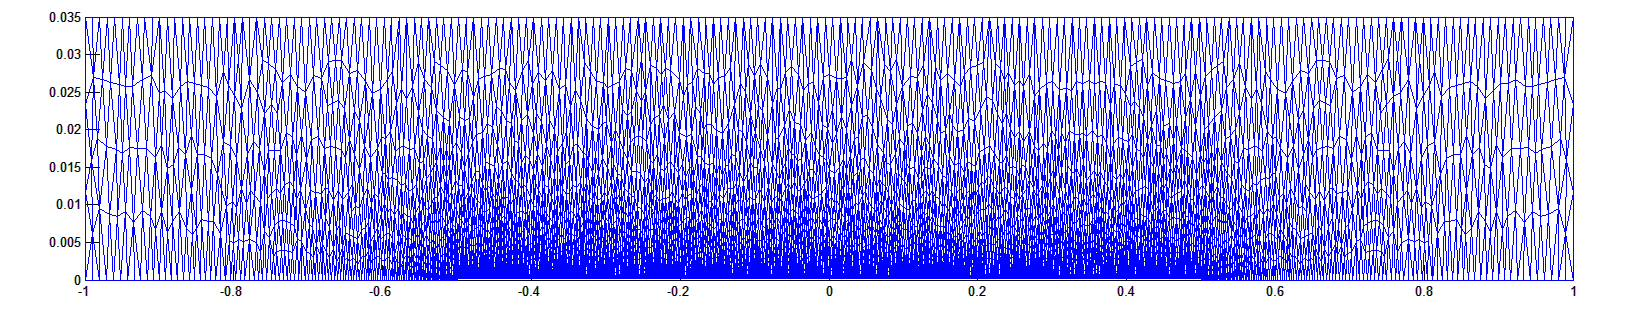
\includegraphics[width=1\textwidth,height=0.25 \textwidth]{images/mesh}
%\caption{Maillage utilisé pour la simulation}
%\label{f mesh}
%\end{figure}

\subsection{Résultats de simulation}
Après simulation, nous observons un profil de potentiel donné par les Figure \ref{f v}.

\begin{figure}[h]
   \begin{minipage}[c]{.32\linewidth}
      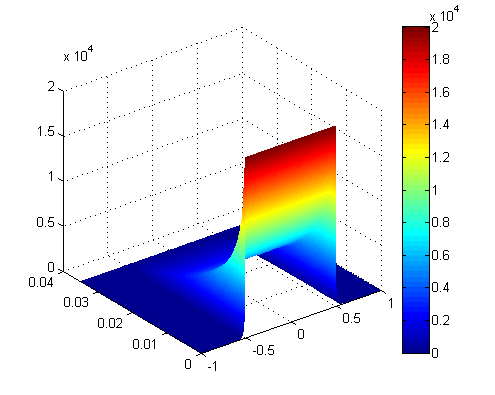
\includegraphics[width=1\textwidth,height=0.8\textwidth]{images/v_3d}
      %\caption{Profil 3D du potentiel}
      \label{f v_3d}
   \end{minipage} \hfill
   \begin{minipage}[c]{.32\linewidth}
      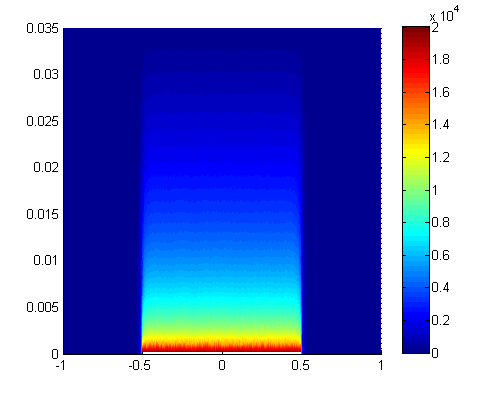
\includegraphics[width=1\textwidth,height=0.8\textwidth]{images/v_xy}
      %\caption{Vue $xOy$ du potentiel}
      \label{f v_xy}
   \end{minipage} \hfill
   \begin{minipage}[c]{.32\linewidth}
      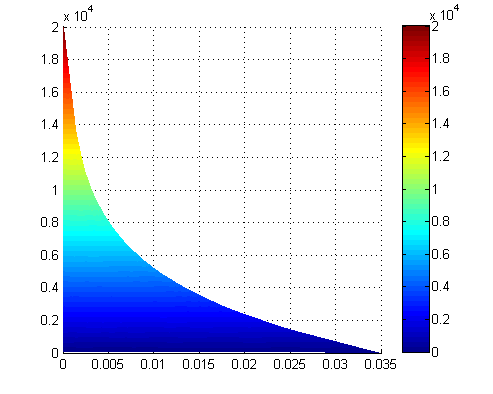
\includegraphics[width=1\textwidth,height=0.8\textwidth]{images/v_yz}
      %\caption{Vue $yOz$ du potentiel}
      \label{f v_yz}
   \end{minipage}
   \caption{Différentes vues du potentiel}
   \label{f v}
\end{figure}


%\begin{figure}[h]
%\centering
%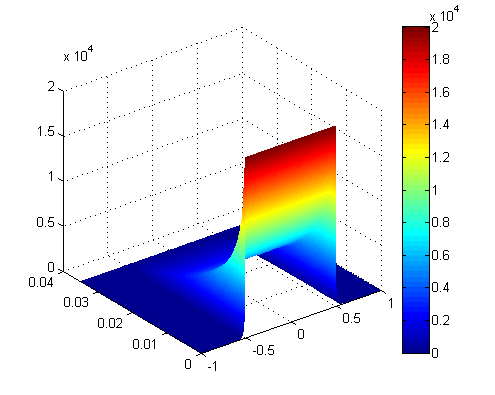
\includegraphics[width=0.5\textwidth,height=0.4\textwidth]{images/v_3d}
%\caption{Profil 3D du potentiel}
%\label{f v_3d}
%\end{figure}

%\begin{figure}[h]
%\centering
%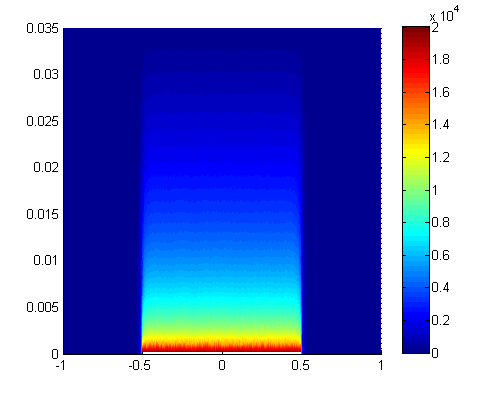
\includegraphics[width=0.5\textwidth,height=0.4\textwidth]{images/v_xy}
%\caption{Vue $xOy$ du potentiel}
%\label{f v_xy}
%\end{figure}

%\begin{figure}[h]
%\centering
%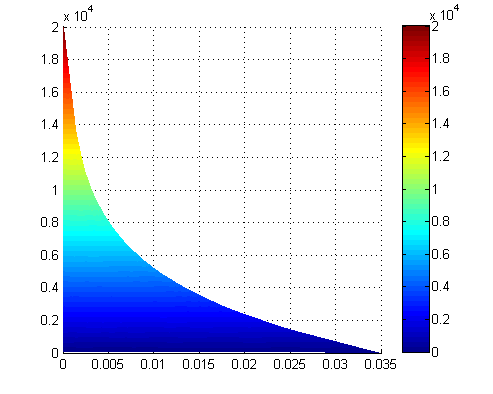
\includegraphics[width=0.5\textwidth,height=0.4\textwidth]{images/v_yz}
%\caption{Vue $yOz$ du potentiel}
%\label{f v_yz}
%\end{figure}


\section{Modélisation des trajectoires}

Une fois que l'on a un programme qui donne la trajectoire de l'électron dans un potentiel et un programme qui détermine le potentiel dans le tube en tenant compte des effets de bord, on peut combiner ces deux programmes pour obtenir la trajectoire de l'électron dans un potentiel déterminé numériquement. La fonction pick.m permet de récupérer le potentiel en un point à l'intérieur du cylindre, ce qui va nous permettre de calculer la trajectoire de l'électron dans le tube.

\section{discussion}



\section{conclusion}
























\end{document}